\section{Business Overview}
Smoking Games started as a small video game developer company. At the beginning they distributed their games through other distributers. After the great hit of a video game called ''full life'', they decided to start distributing their games on their own.\\
In 2010, after 2 years in the development business, Smoking Games became a video game developer and digital distributor enterprise. At the start they only distributed their own games. With the growth of the enterprise Smoking Games got many offers from other game developers to distribute their games. Like this Smoking Games decided that they will distribute also other developers creation in their digital distribution section. At this point the distribution software was named Smoke. \\
2011 was a great year for Smoking Games, the growth of computer gaming in this year helped consolidating the enterprise and Smoke became the gaming platform for everyone. In Smoking Games they didn't think it was enough, as their mission states: "Always creating and innovating". So they took the next step, a cloud service for saving games and cross platform gaming. Playing on two devices always moving forward in a shared game. In the other hand ''full life 3'' was released during this year getting Smoking Games a very good position in the market as a trusted game developer.\\
In 2012, after 4 years in a rented placement the head quarter of Smoking Games moved to a newly owned location. Taking advantage of this growth the whole enterprise grew. It redefined in this year still at the same size of 35 employees fixed plus some external services. Even though the enterprise organization is quite horizontal, the shares and benefits belong to the employees and bosses in the same amount, they keep a minimun organization for political purposes. The hierarchy of the enterprise is the one shown in figure \ref{fig:org_hierarchy}.

\begin{figure}[htpb]\centering
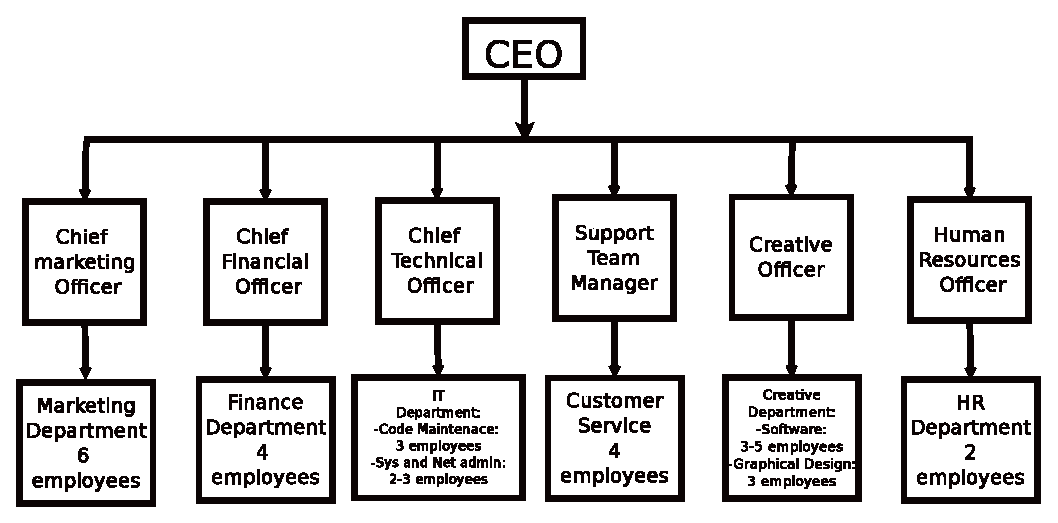
\includegraphics[ width={0.7\textwidth} ] {pictures/Organizational_hierarchy}
\caption{Organizational hierarchy}
\label{fig:org_hierarchy}
\end{figure}
\newpage
\noindent The main source of income for Smoking Games is by selling their own games, those games give a 100\% of the price back. The games produced by other companies are a different story: for every game and developer Smoking Games makes a different contract, going from the 75 to the 50\%money of the solds in the distribution price.\\
Smoking Games is located in a building in Tenerife, Spain. The building next to it is one of the main hubs for telefonica SA, main internet company in Spain. Like this the internet conection is much more ensured. This is important because most of the business of Smoking Games are done over the internet.
